\section[Задачи, вдохновлённые реальностью]{2. Reality-Inspired Problems}

\begin{frame}
\frametitle{Аксиомы выборов}

\usl{2019-7-3A}{На предприятии работают 50 человек, и они выбирают себе начальника. Есть две кандидатуры, Ваня и Даня. Про каждого работника известно заранее, кому он отдаёт предпочтение: 20 человек за Даню, 30 человек за Ваню. \smallskip \\
Голосование проходит по двухтуровой системе: люди делятся на 5 групп по 10 человек, в каждой группе выбирается кандидат, наиболее популярный среди членов этой группы, и затем из 5 ответов выбирается имя, названное большее число раз. \smallskip \\
Разделите работников на группы так, чтобы в большинстве групп выбрали Даню и он победил на выборах, несмотря на изначально меньшее число голосующих за него.}
\end{frame}

\begin{frame}
\frametitle{Аксиомы выборов}

\begin{center} \tikz{
\begin{scope}[rotate=90,scale=1.2]
	\filldraw[fill=gray,draw=gray,opacity=0.32] (0,0) rectangle (1,5);
	\foreach \x in {0,2,5} {\draw[thick, color=gray]
		(0.5 * \x cm, 0) -- (0.5 * \x cm, 5);}
	\foreach \x in {0,10} {\draw[thick, color=gray]
		(0, 0.5 * \x cm) -- (2.5, 0.5 * \x cm);}
	\foreach \x in {1,3,4} {\draw[color=gray, opacity=0.38]
		(0.5 * \x cm, 0) -- (0.5 * \x cm, 5);}
	\foreach \x in {1,...,9} {\draw[color=gray, opacity=0.38]
		(0, 0.5 * \x cm) -- (2.5, 0.5 * \x cm);}

	\draw (0.5,-0.25) node[right]{\large За Даню};
	\draw (1.75,-0.25) node[right]{\large За Ваню};

	\pause
	\begin{scope} [xscale=-1, xshift=-2.5cm]
	\draw[very thick] (0.5,0) -- (0.5,5);
	\draw[very thick] (2.5,1.5) -- ++ (-1,0) --
		++ (0,0.5) -- ++ (-0.5,0) -- ++(0,-2);
	\draw[very thick] (2.5,3.5) -- ++ (-1,0) --
		++ (0,-0.5) -- ++ (-0.5,0) -- ++(0,2);
	\draw[very thick] (2.5,3.5) --
		++ (-1,0) -- ++ (0,-0.5) --
		++ (-0.5,0) -- ++ (0,-1) -- ++ (0.5,0) --
		++ (0,-0.5) -- ++(1,0);
	\end{scope}
\end{scope} } \end{center} \end{frame}

\begin{frame} \frametitle{2020-4-1A, Эскалаторы}

\begin{center} \begin{tabular}{cc}
	\makecell[l]{\newcommand{\staircs}{\filldraw[draw=black,fill=white,fill opacity=0.84]}
\newcommand{\stairwd}{0.305}

\newcommand{\flr}[1]{
     \staircs (0, #1 cm)
	-- ++(-0.5 * \stairwd cm, -1 * \stairwd cm) -- ++(5.8,0)
	-- ++(0.5 * \stairwd cm, \stairwd cm) -- ++(1,2)
	-- ++(0.5 * \stairwd cm, \stairwd cm) -- ++(-5.8,0)
	-- cycle;
}

\newcommand{\stairst}[1]{ \begin{scope}[yshift = #1 cm]
     \staircs (1,2)
	-- ++(0.5 * \stairwd cm, \stairwd cm) -- ++(5.8,4)
	-- ++(-1 * \stairwd cm, -2 * \stairwd cm) -- ++(-5.8,-4)
	-- cycle;
     \staircs (6.3,1)
	-- ++(0.5 * \stairwd cm, \stairwd cm) -- ++(-5.8,4)
	-- ++(-1 * \stairwd cm, -2 * \stairwd cm) -- ++(5.8,-4)
	-- cycle;
     \staircs (0,0)
	-- ++(0.5 * \stairwd cm, \stairwd cm) -- ++(5.8,4)
	-- ++(-1 * \stairwd cm, -2 * \stairwd cm) -- ++(-5.8,-4)
	-- cycle;
     \flr{4}
\end{scope}}

\tikz[scale=0.34]{
	\flr{0} \stairst{0} \stairst{4}
	\stairst{8} \stairst{12}
	\draw[<->] (-0.5 * \stairwd cm, -0.9) -- (5.8 cm - 0.5 * \stairwd cm,-0.9);
	\draw (2.9 cm - 0.5 * \stairwd cm, -0.9) node[below]{12\,м};
	\draw[<->] (5.8 cm + 0.9 cm - 1 * \stairwd cm, -1 * \stairwd cm)
	     -- (6.8 cm + 0.9 cm, 2 cm + \stairwd cm);
	\draw (7.2 cm - 0.5 * \stairwd cm, 1 cm) node[right]{4\,м};
}} &
	\makecell[l]{
		В торговом центре Атмосфера» пять этажей. \\
		Соседние этажи соединяют по три эскалатора. \\
		По утрам администратор запускает каждый \\
		из эскалаторов вверх или вниз. Cпособ \\
		запустить эскалаторы {\it хороший,} если \\
		с любого этажа можно добраться до любого, \\
		не проходя ни по одному из этажей \\
		более 5 метров. Приведите пример; сколько всего \\
		хороших способов ? ($2 \cdot 3^4 = 162$.) \\ \ \\ \ \\}
\end{tabular} \end{center} \end{frame}

\begin{frame} \frametitle{2021-8-5B}
	Рельсовый автобус (одновагонный поезд) длиной $24.5$ метра с четырьмя колёсными парами. Пары расположены на расстоянии $2.7$ метра друг от друга, а между тележками — $14.3$ метра. \begin{center}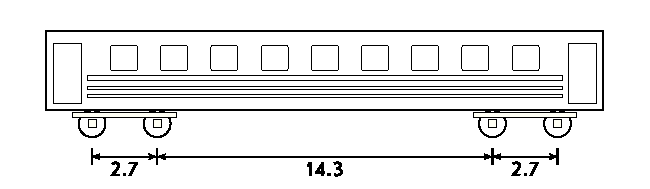
\includegraphics{img/pbvagon}\end{center}

	Можно ли подобрать длины трёх звеньев между длинными плетями так, чтобы стук был равномерным, с одинаковыми паузами между ударами?
\end{frame}
